\chapter{Bole volume\label{chap::bole_v}}

\section{Two sets of equations}

The annual living tree sample surveyed by French NFI is divided into two subsets:  

\begin{itemize}
	\item trees getting girth and height measures ;
	\item *simplified* trees, with girth only measure.
\end{itemize}

First ones are randomly picked from every species group and girth class on each plot and get the following measurements:  

\begin{itemize}
	\item \( c \): tree girth, measured at breast height;
	\item \( h \): total tree height, measured from ground level to the main stem tip;
	\item \( h_{dec} \): tree height from ground level to the terminal cutting level of the log, located at the stem top or at a sudden decrease in stem diameter.
\end{itemize}

Their bole volume is predicted using three-entries allometric equations, as described in \cite{Morneau2016}:  

\begin{equation}
\hat V_{bole} = \frac{c^2 h}{4 \pi \left( 1 - \frac{1{,}3}{h} \right)^2} \hat fnew_{bole}
\label{eq::fnew}
\end{equation}

\[ \hat fnew_{bole} = \left( \alpha + \beta c + \gamma \frac{\sqrt{c}}{h} + f(h_{dec}) + \delta \frac{1}{c^\epsilon} \right) \left[ 1 - b \left( \frac{0{,}07 \pi}{c} \right)^3 \left( 1 - \frac{1{,}3}{h} \right)^3 \right] \]
where \( f(h_{dec}) \) is a function of \( h_{dec} \) among the following:  

\begin{itemize}
	\item \( f(h_{dec}) = fmax \left( \frac{h_{dec}}{h_{dec} + k} \right)^{1 + \rho} \)
	\item \( f(h_{dec}) = \eta ~ln\left( \frac{h_{dec}}{h} \right) \)
	\item \( f(h_{dec}) = \eta ~ln\left( h_{dec} \right) \)
	\item \( f(h_{dec}) = \eta h_{dec} \)
\end{itemize}

(\( \alpha \), \( \beta \), \( \gamma \), \( \eta \), \( fmax \), \( k \), \( \rho \), \( \delta \), \( \epsilon \), \( b \)) are a set of coefficients. Those and \( f(h_{dec}) \) are both depending on the tree species.  
(\( \alpha \), \( \beta \), \( \gamma \), \( \eta \), \( fmax \), \( k \), \( \rho \), \( \delta \)) also depend on the kind of terminal cut of the tree, either the stem top (*regular cut*) or a sudden decrease in stem diameter (*shape cut*).  

As for simplified trees, one refer to the predicted volume of a neighbour tree. One-entry allometric equations are used to fix the girth gap between reference and simplified trees when assigning bole volume to the last.  

\begin{tcolorbox}[breakable, title = Volume imputation]
\begin{equation}
\hat V_{bole}(i) = V_{III}(j) \frac{V_{I}(i)}{V_{I}(j)}
\label{eq::imputation}
\end{equation}
where \( V_{III} \) and \( V_{I} \) are bole volume estimates by three-entries or one-entry allometric equations:  

\begin{itemize}
	\item \( V_{III} = f(c, h, h_{dec}) \)
	\item \( V_{I} = f(c) \)
\end{itemize}

\( j \) is a tree with height measures within the same species group and girth class than the simplified tree \( i \).  
\end{tcolorbox}

Current one-entry allometric equations are built on log transformation:  

\[ V_{I} = \mathrm{e}^{\alpha + \beta ln(c) + \gamma ln(c)^2 + \delta ln(c)^3 + \zeta ln(c)^4 + \eta f(g) + \frac{\sigma^2}{2}} \]
where \( f(g)$ is a function of local basal area.  
(\( \alpha \), \( \beta \), \( \gamma \), \( \delta \), \( \zeta \), \( \eta \), \( \sigma \)) are coefficients depending on the tree species and contextual parameters (ecological area, altitude zone, property regime).  

\section{Motivations for changes}

Regarding three-entries allometric equations, one aim at improving model parcimony. Future species models all share the same formula. Also, fitting rely no more on the kind of terminal cut.  
In relation to it, a decision is to get rid of \( h_{dec} \) entry for trees with regular cut: since 2020, \( h_{dec} \) is no longer measured on that kind of trees and now it has to be assessed by a third-party model. One achieve it by setting down \( h_{dec}' \) as:

\[ h_{dec}' = \begin{cases}
h_{dec} & \text{in case of a shape cut}\\
h & \text{otherwise}
\end{cases} \]

For monitoring stock variations over time, the new coming inventory method will assess tree sample data twice. Tree samples are surveyed a second time, but only tree girth is measured again. So, one-entry allometric equations shall be used to assess tree new volume at second survey given old and new girth, the same way than simplified trees (see \ref{eq::imputation}). For that purpose, one-entry volume equations have to be an increasing function of girth. In particular, an explanatory variable \( f(g) \) involving local basal area, conveying stand competition, has to be questioned.  

The approach of new allometric equations development is detailed in \cite{Gohon2024}.  

\section{New bole models}

Like current equations, future three-entries models are fitted using French NFI data (see \ref{chap::def} 3.). It models a shape coefficient \( fnew_{bole} \) (see \ref{eq::fnew}) an analogous way than \cite{Morneau2016}.  

\[ \hat fnew_{bole} = \alpha + \beta c + \gamma \frac{\sqrt{c}}{h_{dec}'} + \delta \frac{\sqrt{h_{dec}'}}{c^2 h} + \eta \left( 1 - \frac{h_{dec}'}{h} \right) \]
where coefficients (\( \alpha \), \( \beta \), \( \gamma \), \( \delta \), \( \eta \)) only depend on the tree species.  

New one-entry models are fitted to volume estimates of trees with height measures from recent inventory campaigns.  

\[ V_{I} = \mathrm{e}^{\alpha + \beta ln(c) + \gamma ln(c)^2 + \frac{\sigma^2}{2}} \]
where (\( \alpha \), \( \beta \), \( \gamma \), \( \sigma \)) are still depending on the tree species and same contextual parameters (ecological area, altitude zone, property regime).  

New and current models perform similarly.  
Survey estimates (see for instance \ref{fig::estimate_vbole_bygirth} and \ref{fig::estimate_vbole} from \cite{Gohon2024}) are a go-to output to foresee the forthcoming effect of new allometric equations on NFI results. It shows lower volume estimates for small trees and slightly higher volume estimates for bigger trees, and consequently higher volume growth estimates. Differences never exceed confidence intervals.  

\begin{figure}
	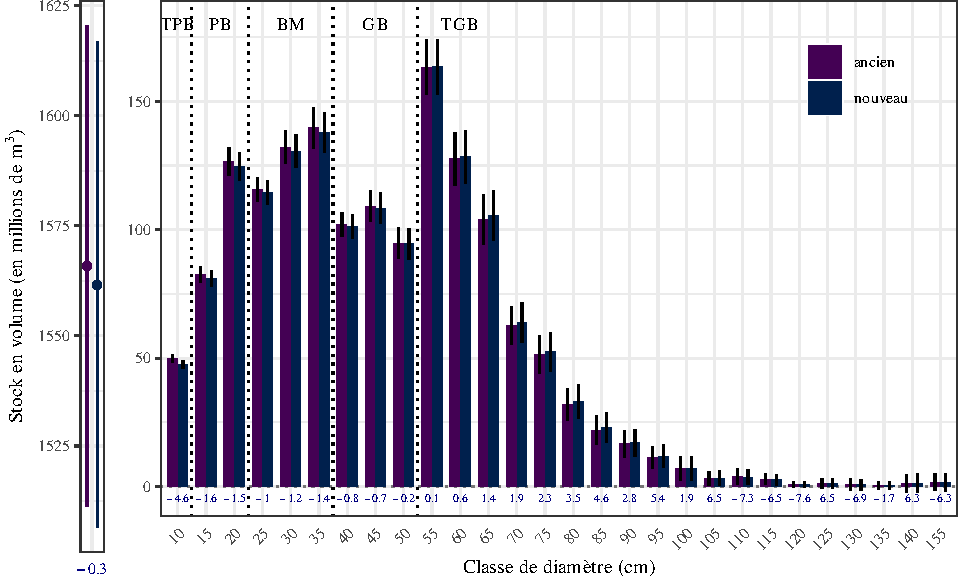
\includegraphics{figure/estimate_vbole_bygirth.pdf}
	\caption{National bole volume estimates for trees with height measures, by rounded girth. \label{fig::estimate_vbole_bygirth}}
\end{figure}

\begin{figure}
	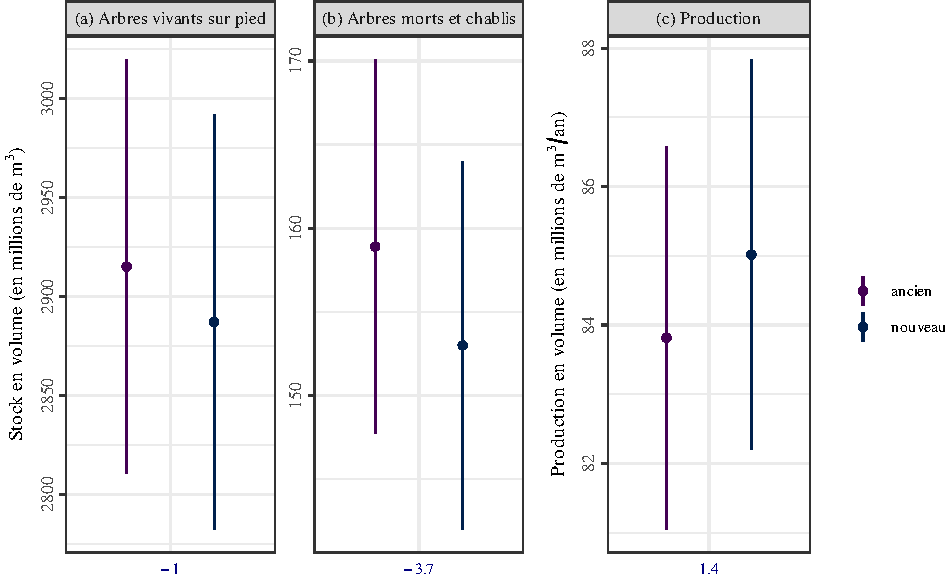
\includegraphics{figure/estimate_vbole.pdf}
	\caption{National bole volume and growth estimates for all living trees and dead trees. \label{fig::estimate_vbole}}
\end{figure}


